\section{Red Flags} % Top level section
\begin{fullwidth}
During the course of the initial interview with Sam's friends, the fraud fighting team identified a number of potential red flags with the HealthComp job opportunity.

\subsection{Email Red Flags}
The email that Sam received contains multiple red flags that indicate that it may be a phishing email. These include:
\begin{itemize}
	\item Numerous grammatical errors \hyperref[sec:NIST Phish Scale]{(NIST Phish Scale Cue Type: Error)}
        \begin{itemize}
            \item Several misspelled words \hyperref[sec:Fig2]{(See Figure 2)}
            \item Several missed commas \hyperref[sec:Fig3]{(See Figure 3)}
            \item Several run on sentences \hyperref[sec:Fig4]{(See Figure 4)}
            \item Discrepancies with how David Bondeson is titled
            \hyperref[sec:Fig5]{(See Figure 5)}
        \end{itemize}
    \item Email address referenced in email is healthcomp.live \hyperref[sec:NIST Phish Scale]{(NIST Phish Scale Cue Type: Technical Indicators)}
        \begin{itemize}
            \item healthcomp.live is not utilized by HealthComp, the company uses healthcomp.com for email communication
            \item The healthcomp.live domain was recently registered
        \end{itemize}
    \item Sender Kellie McDaniel is not listed as a HealthComp employee \hyperref[sec:NIST Phish Scale]{(NIST Phish Scale Cue Type: Technical Indicators)}
	\item Email signed by HealthComp instead of the sender or an HR Representative \hyperref[sec:NIST Phish Scale]{(NIST Phish Scale Cue Type: Language and Content)}
	\item Email is generically addressed to "Candidate" as opposed to Sam \hyperref[sec:NIST Phish Scale]{(NIST Phish Scale Cue Type: Language and Content)}
    \item Utilizes a "verification code" as opposed to applicant name
\end{itemize}

\subsubsection{Grammatical Errors}

\begin{figure*}[H] % Use the figure* environment for full width figures
    \label{sec:Fig2}
    \centering
    
\includegraphics[width=.75\linewidth]{assets/misspelling.png}
    \captionsetup{justification=centering}
    \caption{Misspelling of "fitment". It should just say "fit".}
\end{figure*}

\begin{figure*}[H] % Use the figure* environment for full width figures
    \label{sec:Fig3}
    \centering
    
\includegraphics[width=.75\linewidth]{assets/missedCommas.png}
    \captionsetup{justification=centering}
    \caption{There should be a comma following "\$27/hr" and before "but".}
\end{figure*}

\begin{figure*}[H] % Use the figure* environment for full width figures
    \label{sec:Fig4}
    \centering
    
\includegraphics[width=.75\linewidth]{assets/runon.png}
    \captionsetup{justification=centering}
    \caption{This is a run-on sentence that should be broken up into two or three separate sentences.}
\end{figure*}

\begin{figure*}[H] % Use the figure* environment for full width figures
    \label{sec:Fig5}
    \centering
    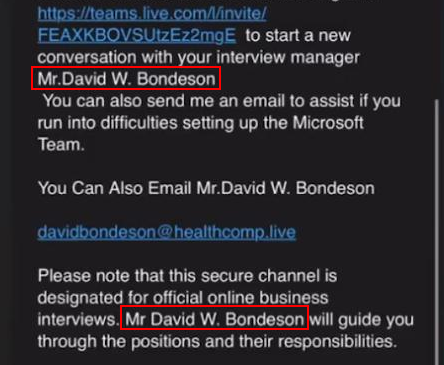
\includegraphics[width=.75\linewidth]{assets/titleerror.png}
    \captionsetup{justification=centering}
    \caption{Discrepancy between "Mr.David W. Bondeson" compared to "Mr David W. Bondeson".}
\end{figure*}

\subsection{Job Red Flags}
The job posting includes various red flags. These include:
\begin{itemize}
	\item Job interview is for 6 different positions
        \begin{itemize}
            \item All jobs have the same pay rate despite different duties and skill levels \hyperref[sec:Fig6]{(See Figure 6)}
            \item All jobs are fully remote and create your own schedule \hyperref[sec:Fig7]{(See Figure 7)}
            \item None of the jobs are listed on the HealthComp careers website \hyperref[sec:Fig8]{(See Figure 8)}
        \end{itemize}
    \item Interview is scheduled through a text based chat instead of phone, video, or in person.
    \item On LinkedIn, David is listed as "Director of Stop Loss Sales", a director is not likely to conduct an interview for an entry level position \hyperref[sec:Fig1]{(See Figure 1)}
\end{itemize}

\subsubsection{Job Posting Evidence}

\begin{figure*}[H] % Use the figure* environment for full width figures
    \label{sec:Fig6}
    \centering
    
\includegraphics[width=.75\linewidth]{assets/positions.png}
    \captionsetup{justification=centering}
    \caption{The email specifies these six job positions as available.}
\end{figure*}

\begin{figure*}[H] % Use the figure* environment for full width figures
    \label{sec:Fig7}
    \centering
    
\includegraphics[width=.75\linewidth]{assets/remoteSched.png}
    \captionsetup{justification=centering}
    \caption{The email specifies all jobs are work-from-home and have custom schedules.}
\end{figure*}

\begin{figure*}[H] % Use the figure* environment for full width figures
    \label{sec:Fig8}
    \centering
    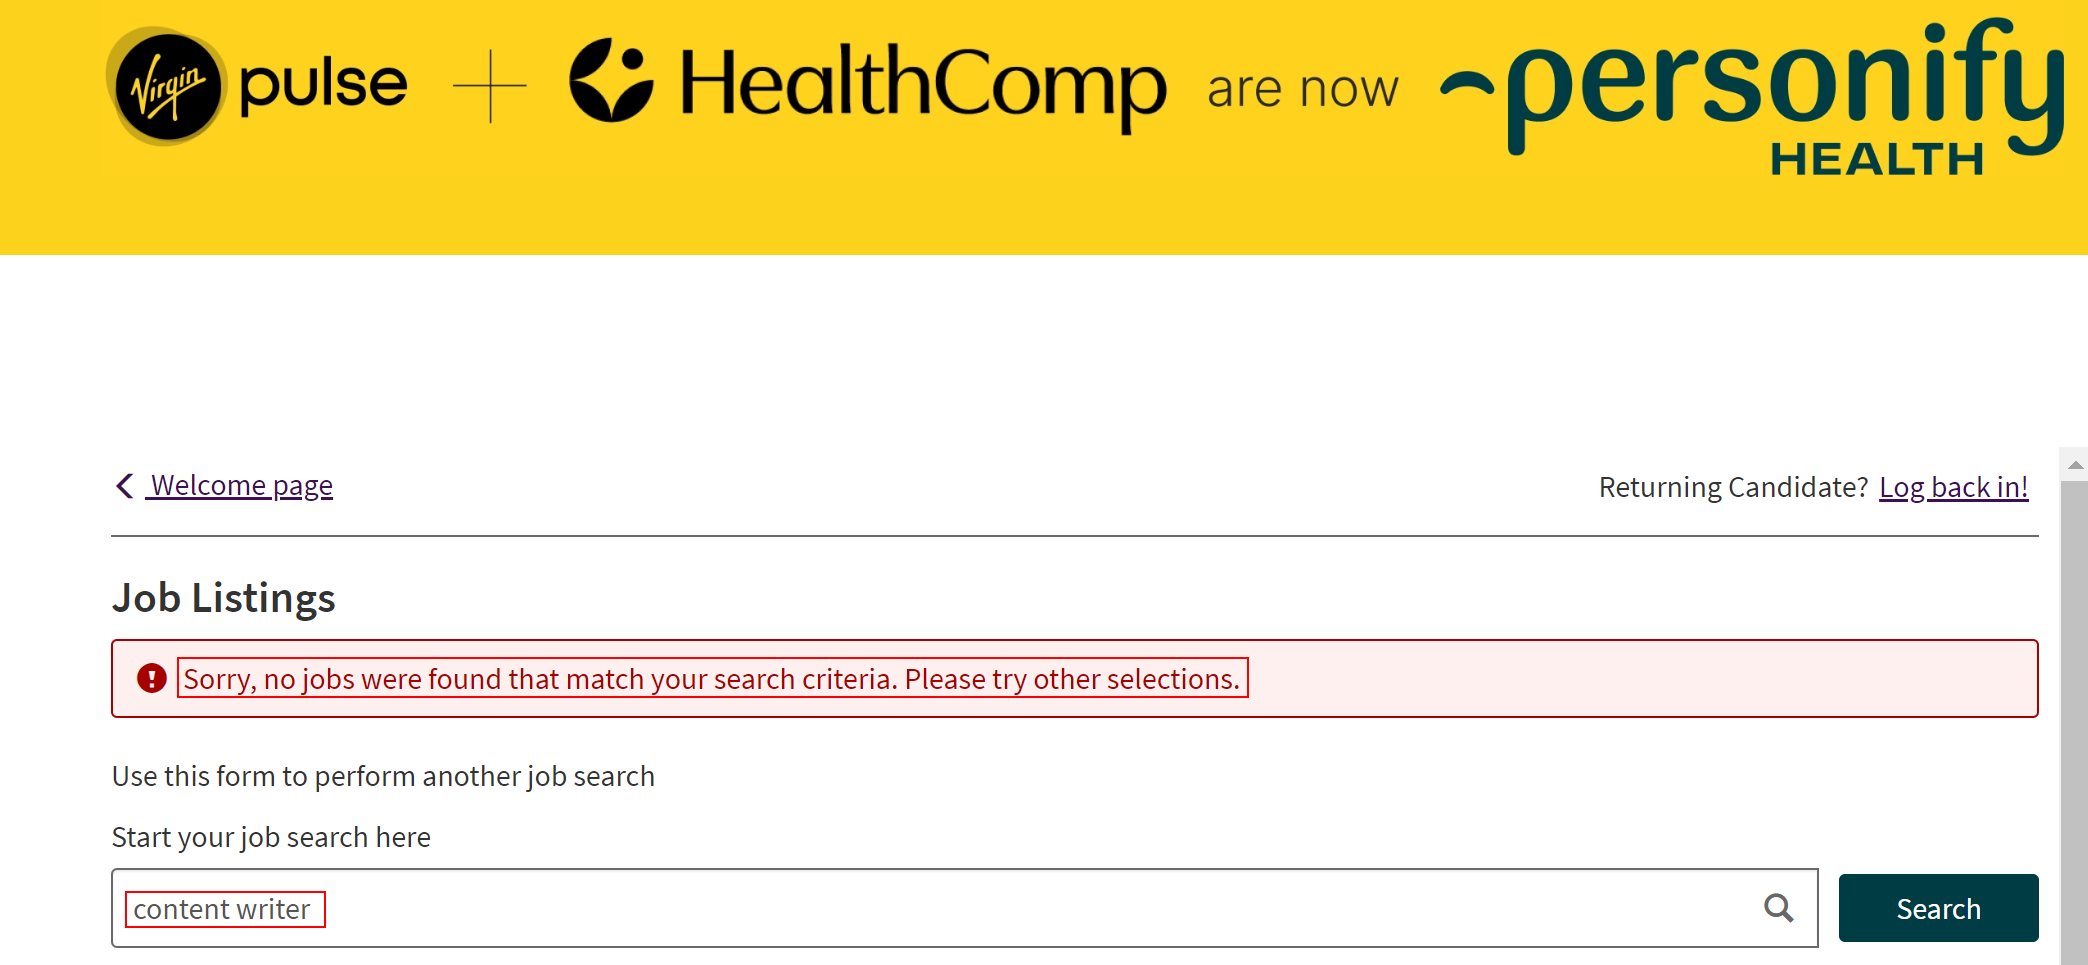
\includegraphics[width=1\linewidth]{assets/realJobPosting.png}
    \captionsetup{justification=centering}
    \caption{The job listings for HealthComp do not have the offered position of content writer available}
\end{figure*}

\subsection{BBB Scam Report}
\label{sec:BBB Scam Report}

The team found a report submitted to the Better Business Bureau which fits the exact description of Sam's interactions with the prospective employer.

\begin{quote}
	\textbf{\LARGE ``}I was sent an email about a potential job offer for HealthComp I then got instructions to conduct an interview on Microsoft Team then they so called hired me and had me fill out paper work including a W4 form that had my ssn number then after that I told them I had finished filling out the paper work and then they started asking if I was going to be using a credit card to accept my payments and I said no then they said I need one so they can process faster then that's when I realized it was a scam\textbf{''}
	
	\hfill--- BBB Scam ID \#772647 \autocite{BBB:2023}
\end{quote}

The BBB Scam Report lists the same davidbondeson@healthcomp.live email address referenced in Sam's interview offer. With this in mind, it's extremely likely that Sam's job opportunity is not legitimate.
\end{fullwidth}